\section{リングイメージング・チェレンコフ検出器}
$(\ref{eq:cherenkov_condition})$式から、荷電粒子の質量$m$と輻射体の屈折率$n$が既知の場合、
チェレンコフ放射が発生する荷電粒子の運動量の閾値$p_t$は$(\ref{eq:cherenkov_momentum_condition})$式のように表される。
\begin{equation}
  \label{eq:cherenkov_momentum_condition}
  p_t = \frac{m}{\sqrt{n^2-1}}
\end{equation}
したがって、荷電粒子の運動量が既知の場合、適切な屈折率の輻射体を用いることで荷電粒子の種類が特定できる。
このように、チェレンコフ放射の有無で粒子識別を行うものを閾値型チェレンコフ検出器という。
これに対し、チェレンコフ光を検出し、チェレンコフ角を測定することにより
$(\ref{eq:cherenkov_angle})$式から粒子の速度を求め、粒子識別を行うものをリングイメージング・チェレンコフ検出器という。
今回は、リングイメージング型のチェレンコフ検出器についての研究を行った。

\subsection{輻射体}
チャームバリオン分光実験では、リングイメージング・チェレンコフ検出器で2--16\space$\si{\GeV / c}$の広い
運動量領域での$\pi/K/p$の粒子識別が必要となるため、2種類の輻射体を用いる。
低運動量の粒子識別には屈折率1.04のエアロゲルを使用し、高運動量の粒子識別には屈折率1.00137の$\rm{C_{4}F_{10}}$を使用する。


\subsection{球面鏡}
図\ref{fig:SphericalMirror1}に球面鏡を使用しない場合のリングイメージング・チェレンコフ検出器の概要図を示す。
チェレンコフ光は荷電粒子の軌跡に沿って発生するため、発生地点によってリングサイズに違いが出る。
球面鏡は平行に入射した光を焦点面に収束する性質があるため、球面鏡を用いてチェレンコフ光を反射させることで、リングを収束することができる。


\begin{figure}[htbp]
  \centering
  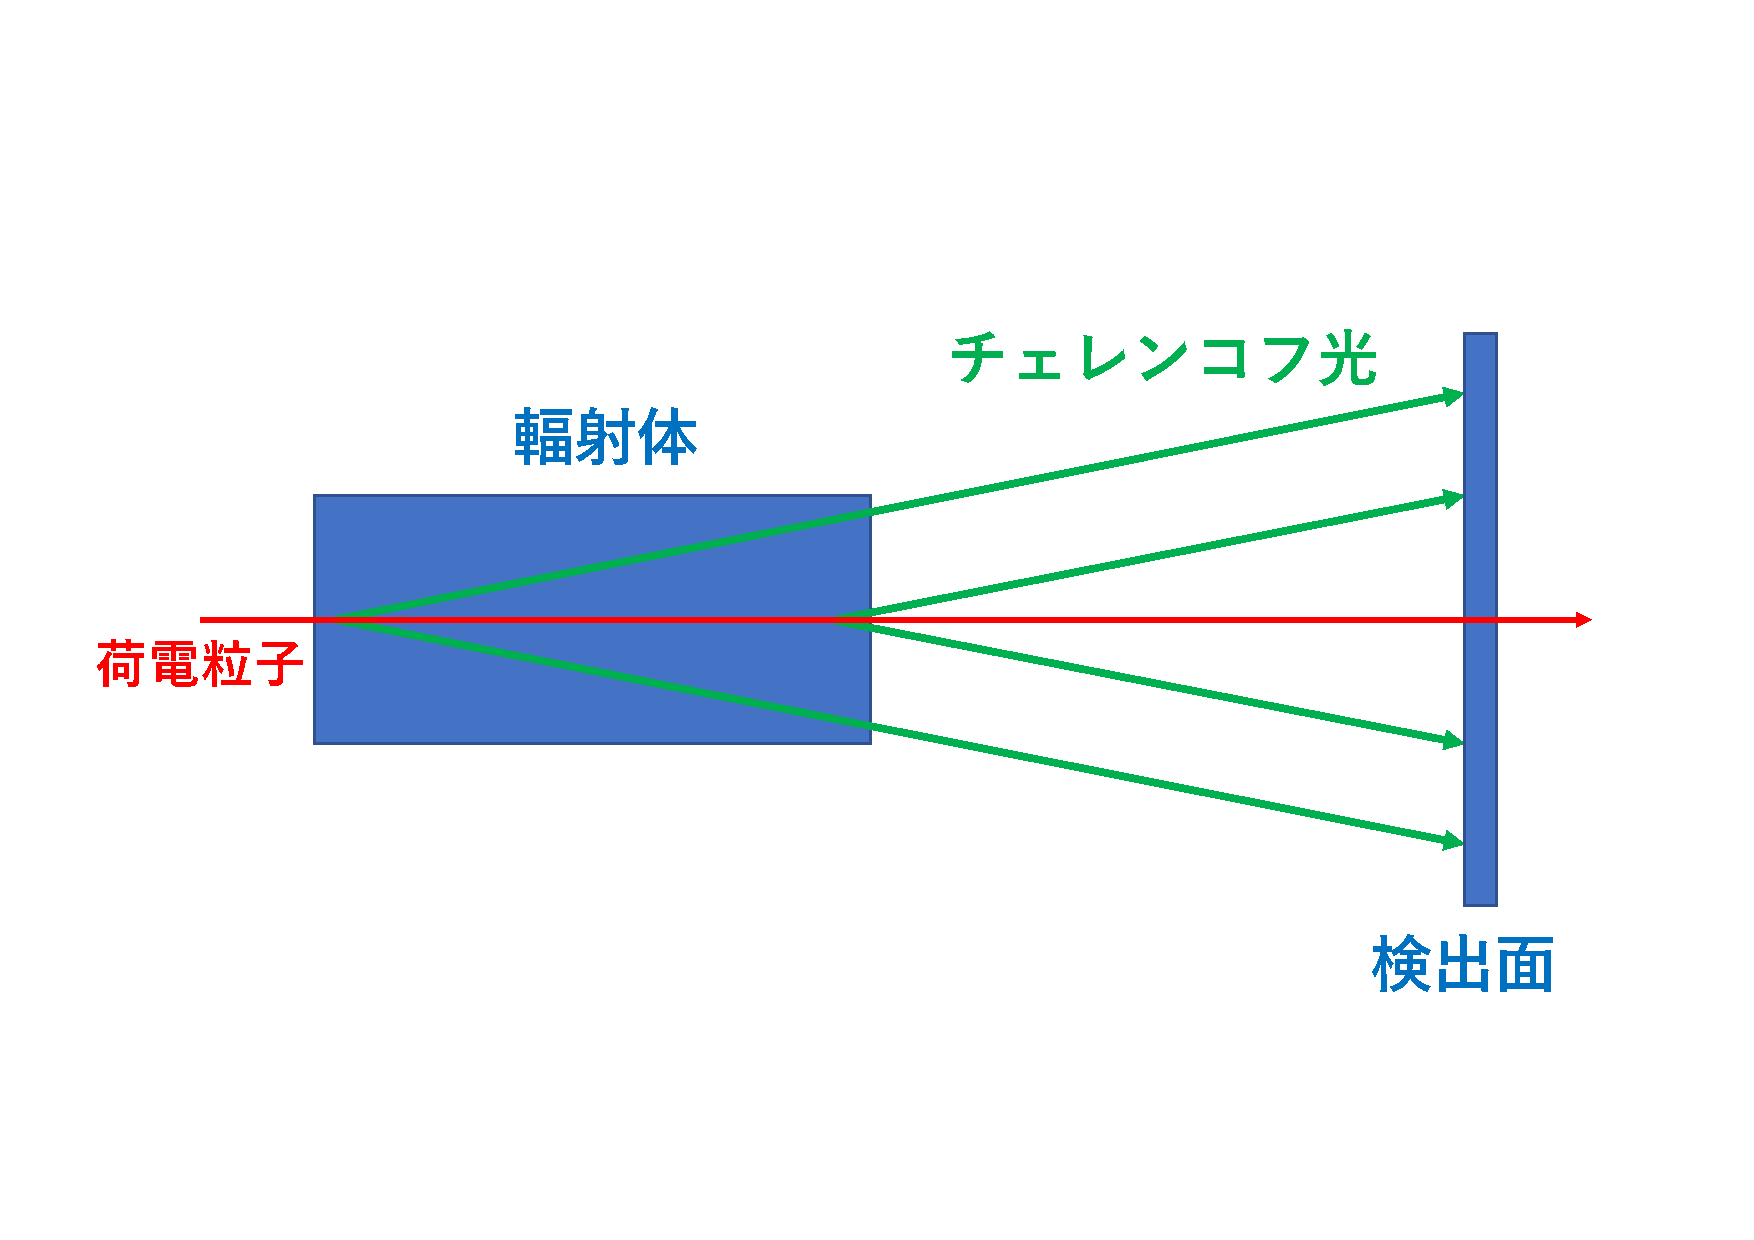
\includegraphics[width=10cm, page=1]{images/chapter2/SphericalMirror.pdf}
  \caption{球面鏡を使用しないリングイメージング・チェレンコフ検出器の概要図。輻射体が厚い場合、チェレンコフ光の発光場所によってリングサイズが変化するため、リングが太くなり分解能が悪化する。}
  \label{fig:SphericalMirror1}
\end{figure}
\begin{figure}[htbp]
  \centering
  \includegraphics[width=10cm, page=2]{images/chapter2/SphericalMirror.pdf}
  \caption{球面鏡を使用したリングイメージング・チェレンコフ検出器の概要図。球面鏡は平行に入射した光を焦点面に収束する性質があるため、リングの幅を幅を小さくすることができる。}
  \label{fig:SphericalMirror2}
\end{figure}

\subsection{光検出器}
チャームバリオン分光実験では、リングイメージング・チェレンコフ検出器の光検出器としてMulti-Pixel Photon Counter(MPPC)\cite{ref8}を使用する。
RICHは磁気スペクトロメーターからの漏れ磁場中に設置するため、磁場の影響を受ける光電子増倍管(PMT)ではなく磁場の影響を受けないMPPCが適している。
一方で、MPPCを使用する際のデメリットとしてDark currentの影響と受光面のサイズがある。
Dark currentとは熱電子によって発生する信号で、光子が入射した際に発生する信号との区別はできない。
Dark currentのレートはMPPCの受光面の面積に比例し、本研究で使用した$\SI{6}{mm}\times\SI{6}{mm}$の受光面だとおよそ$\SI{2}{MHz}$となる。
チェレンコフ光は光量が少ないため、Dark currentが多いと本来のチェレンコフ角を求めることが難しくなる。
この影響に関しては、第4章でのシミュレーションで考察する。
また、MPPCの小さい受光面に対し、RICHで必要となる検出面積は$\SI{2}{m}\times\SI{1}{m}$と大きく
MPPCのみで検出することは難しいため、集光用のコーン型ライトガイドの開発を行った。
コーン型ライトガイドの設計については、第3章で述べる。

\subsection{先行研究による要求性能}
チャームバリオン分光実験におけるRICHは、上流の飛跡検出器で得られた位置情報や運動量情報を用いて
生成粒子の識別を行う。
RICHでは、TOF検出器での測定が難しくなる$\SI{2}{GeV/c}$から$\SI{16}{GeV/c}$までの広い運動量領域で
の$\pi$/K/pの粒子識別を行う。
チャームバリオンの検出感度を十分高くするため、$90\%$以上の検出効率と、$3\%$以下の誤識別率が要求される。
